\documentclass[tikz,border=8pt]{standalone}
% Shared look for every TikZ diagram. Load with \input{../../tools/tikz-style.tex}
\usepackage[T1]{fontenc}
\usepackage{lmodern}
\renewcommand{\sfdefault}{lmr}  % diagrams use the same serif as the text
\usetikzlibrary{arrows.meta, positioning, shapes.geometric, calc, fit, backgrounds}
\definecolor{cblue}{HTML}{4C78A8}
\definecolor{corange}{HTML}{F58518}
\definecolor{cgreen}{HTML}{54A24B}
\definecolor{cred}{HTML}{E45756}
\definecolor{cpurple}{HTML}{B279A2}
\definecolor{cgrey}{HTML}{6B6B6B}
\tikzset{
  every picture/.style={font=\sffamily, line width=1.2pt},
  box/.style={draw=#1, fill=#1!12, rounded corners=4pt, align=center, inner sep=7pt, minimum height=1.1cm},
  box/.default=cgrey,
  arrow/.style={-{Stealth[length=3mm]}, draw=cgrey, line width=1.4pt},
  title/.style={font=\sffamily\bfseries\Large},
  note/.style={font=\sffamily\small, text=cgrey, align=center},
}
\AtBeginDocument{\hyphenpenalty=10000 \exhyphenpenalty=10000}

\begin{document}
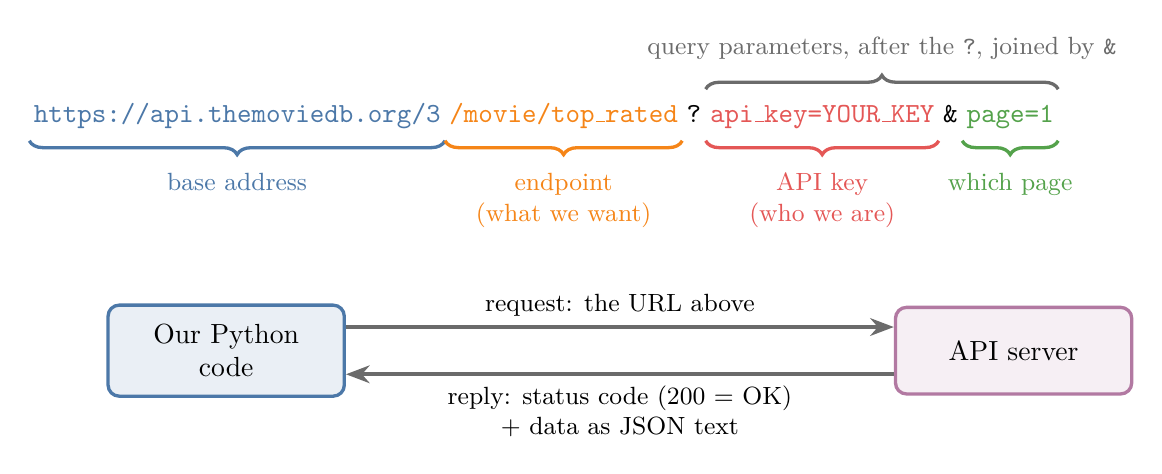
\begin{tikzpicture}[part/.style={font=\ttfamily, inner sep=1pt, anchor=base west}]
  % the URL, cut into its parts
  \node[part, text=cblue] (base) at (0,0) {https://api.themoviedb.org/3};
  \node[part, text=corange] (end) at (base.base east) {/movie/top\_rated};
  \node[part] (q) at (end.base east) {?};
  \node[part, text=cred] (key) at (q.base east) {api\_key=YOUR\_KEY};
  \node[part] (amp) at (key.base east) {\&};
  \node[part, text=cgreen] (pg) at (amp.base east) {page=1};
  \draw[decorate, decoration={brace, mirror, amplitude=5pt}, draw=cblue] ($(base.south west)+(0,-0.1)$) -- ($(base.south east)+(0,-0.1)$) node[midway, below=8pt, note, text=cblue]{base address};
  \draw[decorate, decoration={brace, mirror, amplitude=5pt}, draw=corange] ($(end.south west)+(0,-0.1)$) -- ($(end.south east)+(0,-0.1)$) node[midway, below=8pt, note, text=corange]{endpoint\\(what we want)};
  \draw[decorate, decoration={brace, mirror, amplitude=5pt}, draw=cred] ($(key.south west)+(0,-0.1)$) -- ($(key.south east)+(0,-0.1)$) node[midway, below=8pt, note, text=cred]{API key\\(who we are)};
  \draw[decorate, decoration={brace, mirror, amplitude=5pt}, draw=cgreen] ($(pg.south west)+(0,-0.1)$) -- ($(pg.south east)+(0,-0.1)$) node[midway, below=8pt, note, text=cgreen]{which page};
  \draw[decorate, decoration={brace, amplitude=5pt}, draw=cgrey] ($(key.north west)+(0,0.15)$) -- ($(pg.north east)+(0,0.15)$) node[midway, above=7pt, note]{query parameters, after the \texttt{?}, joined by \texttt{\&}};
  % request and reply
  \node[box=cblue, minimum width=3.0cm] (py) at (2.5,-2.9) {Our Python\\code};
  \node[box=cpurple, minimum width=3.0cm] (srv) at (12.5,-2.9) {API server};
  \draw[arrow] ($(py.east)+(0,0.3)$) -- node[above, font=\sffamily\small]{request: the URL above} ($(srv.west)+(0,0.3)$);
  \draw[arrow] ($(srv.west)+(0,-0.3)$) -- node[below, font=\sffamily\small, align=center]{reply: status code (200 = OK)\\+ data as JSON text} ($(py.east)+(0,-0.3)$);
\end{tikzpicture}
\end{document}
